\documentclass{rho-class/rho}
\pagestyle{plain}

% override Rho margins (geometry already loaded by the class)
\geometry{a4paper, margin=2.5cm}

% override Rho caption size
\usepackage{caption}
\usepackage{capt-of} % for \captionof
\captionsetup{
  font=normal,
  labelfont=bf,
  labelsep=period
}

% set up for long tables
\usepackage{longtable}
\usepackage{booktabs}
\usepackage{multirow}

% avoid header clipping with fancyhdr
\setlength{\headheight}{14pt}

% --- subtitle support for Rho (Rho defines \@maketitle without a subtitle hook) ---
\makeatletter
\newcommand{\subtitle}[1]{\gdef\@subtitle{#1}}
\providecommand{\@subtitle}{} % default empty
\makeatother

% patch \@maketitle to print subtitle below title
\usepackage{etoolbox}
\makeatletter
\patchcmd{\@maketitle}
  {{\RaggedRight\color{rhocolor}\sffamily\bfseries\fontsize{16}{22}\selectfont\@title\par}}
  {{\RaggedRight\color{rhocolor}\sffamily\bfseries\fontsize{16}{22}\selectfont\@title\par}%
   \ifx\@subtitle\@empty\else
        \vskip8pt
        {\RaggedRight\sffamily\bfseries\fontsize{13}{16}\selectfont\color{black}\@subtitle\par}%
   \fi}
  {}{}
\makeatother

% figure/table numbering for SI
\renewcommand{\thefigure}{S\arabic{figure}}
\renewcommand{\thetable}{S\arabic{table}}

\title{Supplementary Information For:}
\subtitle{Genome-Wide Analysis Reveals Altitude-Associated Divergence in a Color-Polymorphic Insect}
\author{}
\date{}

\begin{document}

% Force single-column layout for the whole document
\onecolumn

\maketitle

\section{Methods}
    \subsection{RAD Library Preparation}
        RAD libraries were prepared following the biotinylated adapter protocol of \cite{Ali2016} with minor modifications. Briefly, genomic DNA (~50 ng per sample) was digested with SbfI-HF, ligated to biotinylated adapters containing 8-bp Hamming barcodes, and pooled after ligation. The pooled DNA was sheared to 300–500 bp fragments using a Bioruptor NGS sonicator and size distribution was verified by fragment analysis. RAD-tagged fragments were isolated using streptavidin magnetic beads (Dynabeads M-280), and the captured DNA was released by a secondary SbfI-HF digestion. Purified fragments were then used as input for library construction with the NEBNext Ultra DNA Library Prep Kit for Illumina without protocol modification. Libraries were quantified by qPCR, quality-checked on a Bioanalyzer, and sequenced as paired-end reads on an Illumina HiSeq 4000 platform.

    \subsection{RAD Library Preparation}
        For de novo discovery and extension of RAD loci, we utilized custom PERL scripts, Novoalign alignment software, and the PRICE genome assembler (\cite{Ruby2013PRICE}). We used two individuals from the CAYMY population outside of the Fırtına Valley of I. rizeensis to identify unique RAD-loci. In brief, 88 bp forward reads were trimmed to 80 bp from the 3' end, quality filtered using a read-level probability threshold of $\geq$ 0.80\ estimated accuracy, and concatenated into a single FASTA file. This FASTA file was indexed using Novoalign and aligned against itself to produce a pairwise alignment map. The map included scores for both internal (within-individual) and external (between-individual) alignments (\cite{Miller2012SalmonidHaplotype}). Distinct loci were determined using the following criteria: a maximum alignment score of 30 between sequences within a locus; alignments exceeding a score of 90 or perfect internal alignments were excluded; single-occurrence sequences were ignored unless they perfectly matched a sequence occurring in multiple instances externally; and each locus had to include at least one sequence from two different individuals. 
        
        Identified RAD loci were then extended into longer contigs using PRICE. Paired-end read data were used to iteratively extend each RAD locus into contigs. For each locus, three input files were created: (1) a template file with the 80 bp RAD locus and its restriction site restored, (2) a forward read file with all exact matches to the RAD locus, and (3) a reverse read file with paired reads. To prevent upstream extension, a 100 bp poly-A sequence was added before the restriction site in the template file. These files were processed in PRICE using the following parameters: 300 bp insert size, 95\% minimum sequence identity, 40 nt minimum overlap length (-mol 40), and 80\% sequence identity threshold (-mpi 80). PRICE was set to extend contigs in a single cycle (-nc 1) with a 100\% target mode (-target 100). The resulting extended RAD contigs will then serve as a de novo partial genome reference for subsequent analyses.

\printbibliography

\clearpage

\section{Tables}

\setlength{\LTcapwidth}{\textwidth}
\setlength{\LTleft}{0pt}
\setlength{\LTright}{0pt}
\renewcommand{\arraystretch}{1.08}
\small

\begin{longtable}{l r r r r r r}
\captionsetup{justification=raggedright,singlelinecheck=false}
\caption{Alignment statistics for sequenced individuals. Values are shown for total reads, mapped reads, paired \& mated reads, properly aligned reads, and percent aligned. Individuals in \textbf{bold} had low alignment rates and were excluded from downstream analyses.}
\label{tab:S1}\\

\toprule
Individual & Altitude (m) & Total reads & Mapped reads & Paired \& mated & Properly aligned & \% aligned \\
\midrule
\endfirsthead

\multicolumn{7}{l}{\textbf{Table \thetable} (continued).}\\
\toprule
Individual & Altitude (m) & Total reads & Mapped reads & Paired \& mated & Properly aligned & \% aligned \\
\midrule
\endhead

\midrule
\multicolumn{7}{r}{Continued on next page}\\
\endfoot

\bottomrule
\endlastfoot

IST06\_010          & 450           & 17699665          & 13651474         & 12863816         & 10620563         & 77          \\
IST06\_011          & 450           & 26976950          & 19884407         & 18638649         & 15163675         & 73          \\
IST06\_012          & 450           & 16245005          & 12497863         & 11751688         & 9643402          & 76          \\
IST06\_014          & 450           & 17430558          & 13399937         & 12622347         & 10408325         & 76          \\
IST06\_015          & 450           & 10442391          & 7743033          & 7285646          & 5973732          & 74          \\
IST06\_016          & 450           & 16715690          & 12897325         & 12147188         & 9975883          & 77          \\
IST06\_018          & 450           & 10848723          & 8381111          & 7909968          & 6541399          & 77          \\
PLVYL\_002          & 850           & 6976605           & 5418660          & 5175505          & 4470602          & 77          \\
\textbf{PLVYL\_003} & \textbf{850}  & \textbf{19612190} & \textbf{1898088} & \textbf{1743146} & \textbf{1547493} & \textbf{9}  \\
PLVYL\_014          & 850           & 9449402           & 7177658          & 6771970          & 5591035          & 75          \\
PLVYL\_016          & 850           & 7391430           & 5734330          & 5436938          & 4558937          & 77          \\
PLVYL\_017          & 850           & 10828819          & 8241483          & 7770952          & 6423011          & 76          \\
PLVYL\_018          & 850           & 6534559           & 5114747          & 4882470          & 4191993          & 78          \\
PLVYL\_039          & 850           & 16229237          & 12395271         & 11703801         & 9714141          & 76          \\
IST12\_001          & 900           & 4271052           & 3340688          & 3207430          & 2830601          & 78          \\
IST12\_002          & 900           & 4997360           & 3916977          & 3755619          & 3282121          & 78          \\
IST12\_003          & 900           & 11929527          & 9285710          & 8879229          & 7717793          & 77          \\
IST12\_004          & 900           & 3955474           & 3090713          & 2965469          & 2602165          & 78          \\
IST12\_006          & 900           & 3321161           & 2579615          & 2488134          & 2229783          & 77          \\
IST12\_007          & 900           & 4695955           & 3665321          & 3524147          & 3111008          & 78          \\
IST12\_013          & 900           & 2804691           & 2216449          & 2138677          & 1906883          & 79          \\
IST13\_001          & 1000          & 2226307           & 1752410          & 1674746          & 1443594          & 78          \\
IST13\_002          & 1000          & 3504015           & 2645249          & 2534252          & 2236277          & 75          \\
IST13\_003          & 1000          & 7221678           & 5677734          & 5423570          & 4687285          & 78          \\
IST13\_004          & 1000          & 7692415           & 6086540          & 5836503          & 5068738          & 79          \\
IST13\_005          & 1000          & 6230093           & 4789041          & 4538951          & 3815729          & 76          \\
IST13\_006          & 1000          & 16455730          & 12750280         & 12113527         & 10309764         & 77          \\
IST13\_007          & 1000          & 10117429          & 7739327          & 7398278          & 6442066          & 76          \\
IST14\_018          & 1100          & 8218523           & 6407026          & 6125430          & 5298815          & 77          \\
IST14\_019          & 1100          & 4019398           & 3090422          & 2942185          & 2527816          & 76          \\
IST14\_020          & 1100          & 5126165           & 3981817          & 3815789          & 3331962          & 77          \\
IST14\_021          & 1100          & 7856076           & 6065814          & 5778016          & 4954806          & 77          \\
IST14\_023          & 1100          & 4887089           & 3765392          & 3577413          & 3043257          & 77          \\
IST14\_024          & 1100          & 4877501           & 3579320          & 3413060          & 2946215          & 73          \\
IST14\_025          & 1100          & 5717340           & 4412226          & 4193031          & 3559989          & 77          \\
CANCK\_007          & 1200          & 1880294           & 1457202          & 1394817          & 1212354          & 77          \\
CANCK\_00D          & 1200          & 3713753           & 2872027          & 2751031          & 2404263          & 77          \\
CANCK\_010          & 1200          & 4135115           & 3166137          & 3022983          & 2615446          & 76          \\
CANCK\_011          & 1200          & 4612920           & 3526001          & 3381866          & 2987618          & 76          \\
CANCK\_013          & 1200          & 2277848           & 1746437          & 1665093          & 1434526          & 76          \\
PIKNK\_001          & 1300          & 4069761           & 3183373          & 3028623          & 2572275          & 78          \\
PIKNK\_002          & 1300          & 7487941           & 5883319          & 5597231          & 4739650          & 78          \\
PIKNK\_003          & 1300          & 3325238           & 2586887          & 2471425          & 2132175          & 77          \\
\textbf{PIKNK\_004} & \textbf{1300} & \textbf{64233}    & \textbf{38493}   & \textbf{36924}   & \textbf{33463}   & \textbf{59} \\
PIKNK\_005          & 1300          & 7536536           & 5974430          & 5696328          & 4856381          & 79          \\
\textbf{PIKNK\_006} & \textbf{1300} & \textbf{736149}   & \textbf{581574}  & \textbf{558099}  & \textbf{486683}  & \textbf{79} \\
PIKNK\_007          & 1300          & 8548980           & 6971746          & 6703654          & 5812480          & 81          \\
ELEVT\_001          & 1900          & 13384596          & 10270600         & 9794359          & 8389109          & 76          \\
ELEVT\_002          & 1900          & 6424299           & 4969309          & 4758912          & 4135826          & 77          \\
ELEVT\_003          & 1900          & 8368249           & 6381673          & 6077200          & 5196714          & 76          \\
ELEVT\_005          & 1900          & 5929210           & 4525720          & 4324083          & 3733509          & 76          \\
ELEVT\_006          & 1900          & 5947741           & 4576900          & 4359669          & 3733874          & 76          \\
ELEVT\_007          & 1900          & 5137387           & 3986262          & 3808410          & 3278853          & 77          \\
ELEVT\_008          & 1900          & 14132519          & 11007028         & 10462548         & 8829452          & 77          \\
VRCNK\_002          & 2000          & 8404877           & 6483918          & 6120179          & 5048115          & 77          \\
VRCNK\_003          & 2000          & 8398520           & 6542944          & 6195922          & 5179307          & 77          \\
VRCNK\_005          & 2000          & 22161984          & 17123696         & 16114630         & 13222280         & 77          \\
VRCNK\_006          & 2000          & 7729703           & 5983161          & 5649487          & 4689242          & 77          \\
VRCNK\_008          & 2000          & 3536717           & 2746294          & 2609601          & 2217975          & 77          \\
VRCNK\_009          & 2000          & 14897065          & 11322775         & 10675696         & 8826062          & 76          \\
VRCNK\_010          & 2000          & 15177279          & 11592817         & 10884049         & 8835145          & 76          \\
KALEK\_001          & 2100          & 7970825           & 6252403          & 5935582          & 5010067          & 78          \\
KALEK\_002          & 2100          & 10546009          & 8090899          & 7648716          & 6399616          & 76          \\
KALEK\_003          & 2100          & 14096848          & 10898078         & 10298291         & 8553754          & 77          \\
KALEK\_004          & 2100          & 13550051          & 10481954         & 9889982          & 8195928          & 77          \\
KALEK\_005          & 2100          & 4476058           & 3526383          & 3366569          & 2895995          & 78          \\
KALEK\_007          & 2100          & 6228353           & 4868267          & 4622842          & 3906316          & 78          \\
KALEK\_008          & 2100          & 15403968          & 11878531         & 11193509         & 9241305          & 77          \\
CKLYU\_001          & 2300          & 10299538          & 7884366          & 7480795          & 6334991          & 76          \\
CKLYU\_002          & 2300          & 10733082          & 8277139          & 7831688          & 6549889          & 77          \\
CKLYU\_004          & 2300          & 12319539          & 9517809          & 9009467          & 7552610          & 77          \\
CKLYU\_006          & 2300          & 9480774           & 7296626          & 6898170          & 5745462          & 76          \\
CKLYU\_007          & 2300          & 7163626           & 5628767          & 5372965          & 4622561          & 78          \\
CKLYU\_008          & 2300          & 10799409          & 8507187          & 8103852          & 6914081          & 78          \\
\textbf{CKLYU\_010} & \textbf{2300} & \textbf{24236}    & \textbf{15408}   & \textbf{14714}   & \textbf{13148}   & \textbf{63} \\
\addlinespace[2pt]
\midrule
\addlinespace[2pt]
CAYMY\_002          & 2000          & 13200887          & 10515887         & 10001028         & 8466644          & 79          \\
CAYMY\_004          & 2000          & 18003387          & 14233575         & 13534679         & 11462426         & 79          \\

\end{longtable}
\normalsize

\vspace{1.5\baselineskip} % increase/decrease as you like (e.g., 1, 2, 3 baselines)

\setcounter{table}{1} % ensures this becomes Table S2

\begin{table}[ht]
\small
\begin{flushleft}
\begin{minipage}{0.56\textwidth} % match table width
\captionsetup{
  justification=raggedright,
  singlelinecheck=false,
  width=\linewidth
}
\caption{Summary of per-population missing genotype rates across all 92{,}047 high-quality SNPs. Values represent the mean and standard deviation of missingness per individual within each elevation-defined population.}
\label{tab:S2}

\begin{tabular}{l c cc c}
\toprule
Altitude (m) & No. Indv & \multicolumn{2}{c}{Percent Missing} & No. Loci \\
\cmidrule(lr){3-4}
 &  & mean & std.\ dev. &  \\
\midrule
450  & 7 & 0.23 & 0.16 & 92{,}047 \\
850  & 7 & 0.20 & 0.17 & 92{,}047 \\
900  & 5 & 0.39 & 0.24 & 92{,}047 \\
1000 & 5 & 0.19 & 0.18 & 92{,}047 \\
1100 & 7 & 0.14 & 0.14 & 92{,}047 \\
1200 & 7 & 0.16 & 0.15 & 92{,}047 \\
1300 & 7 & 0.15 & 0.15 & 92{,}047 \\
1900 & 6 & 0.13 & 0.15 & 92{,}047 \\
2000 & 7 & 0.12 & 0.13 & 92{,}047 \\
2100 & 6 & 0.14 & 0.15 & 92{,}047 \\
2300 & 7 & 0.24 & 0.19 & 92{,}047 \\
\bottomrule
\end{tabular}
\end{minipage}
\end{flushleft}
\normalsize
\end{table}

\begin{table}[ht]
\small
\begin{flushleft}
\begin{minipage}{0.68\textwidth} % tweak (0.85–0.95) to match your preferred table width
\captionsetup{
  justification=raggedright,
  singlelinecheck=false,
  width=\linewidth
}
\caption{Genome-wide mean nucleotide diversity (Theta Pi) for neutral and adaptive loci for \textit{I. rizeensis} along an altitudinal gradient in the Fırtına Valley. A paired t-test was performed to assess differences between neutral and adaptive genetic diversity at each altitude.}
\label{tab:S3}

\begin{tabular}{l cc r r r}
\toprule
\multirow{2}{*}{Altitude (m)} & \multicolumn{2}{c}{Mean Theta Pi per site} & \multirow{2}{*}{t\_statistic} & \multirow{2}{*}{df} & \multirow{2}{*}{p value} \\
\cmidrule(lr){2-3}
 & Adaptive loci & Neutral loci &  &  &  \\
\midrule
450  & 0.0645 & 0.0647 & -0.2502 & 963.0000 & 0.8025 \\
850  & 0.0637 & 0.0653 & -1.8726 & 966.0000 & 0.0614 \\
900  & 0.0609 & 0.0631 & -3.0685 & 956.0000 & \textbf{0.0022} \\
1000 & 0.0627 & 0.0639 & -1.4730 & 962.0000 & 0.1411 \\
1100 & 0.0611 & 0.0630 & -2.5397 & 961.0000 & \textbf{0.0113} \\
1200 & 0.0586 & 0.0614 & -4.1246 & 962.0000 & \textbf{< 0.001} \\
1300 & 0.0625 & 0.0646 & -2.6073 & 956.0000 & \textbf{0.0093} \\
1900 & 0.0615 & 0.0637 & -2.7005 & 959.0000 & \textbf{0.0070} \\
2000 & 0.0622 & 0.0626 & -0.5220 & 965.0000 & 0.6018 \\
2100 & 0.0622 & 0.0633 & -1.2400 & 957.0000 & 0.2153 \\
2300 & 0.0634 & 0.0644 & -1.0962 & 957.0000 & 0.2733 \\
\bottomrule
\end{tabular}

\end{minipage}
\end{flushleft}
\normalsize
\end{table}


\setlength{\LTcapwidth}{\textwidth}
\setlength{\LTleft}{0pt}
\setlength{\LTright}{0pt}
\renewcommand{\arraystretch}{1.05}
\small

\begin{longtable}{l r l c c r r r c l}
\captionsetup{justification=raggedright,singlelinecheck=false}
\caption{List of loci significantly associated with altitude (LRT $>$ 24.07) in \textit{I. rizeensis} as revealed by genome-wide association studies. For each RAD locus, the contig identifier (RAD-contig), SNP position (Pos), SNP type (Adaptive/Neutral), major (Maj) and minor (Min) alleles, minor allele frequency (MAF), sample size ($N$), LRT statistic (LRT), genotype counts for wild-type (WT), heterozygous (HE), and homozygous (HO), and the inferred allelic frequency trend along the altitudinal gradient are reported. Loci also significantly associated with colour discrimination are shown in \textbf{bold}.}
\label{tab:S4}\\

\toprule
RAD-contig & Pos & Type & Maj & Min & MAF & $N$ & LRT & WT/HE/HO & Trend \\
\midrule
\endfirsthead

\multicolumn{10}{l}{\textbf{Table \thetable} (continued).}\\
\toprule
RAD-contig & Pos & Type & Maj & Min & MAF & $N$ & LRT & WT/HE/HO & Trend \\
\midrule
\endhead

\midrule
\multicolumn{10}{r}{Continued on next page}\\
\endfoot

\bottomrule
\endlastfoot

R004174             & 136          & Adaptive          & T            & C            & 0.231          & 71          & 24.805          & 32/29/0           & Increasing          \\
R009081             & 18           & Adaptive          & T            & C            & 0.206          & 71          & 26.754          & 39/28/0           & Decreasing          \\
R009667             & 81           & Adaptive          & C            & T            & 0.169          & 71          & 25.624          & 44/21/0           & Increasing          \\
R010003             & 49           & Adaptive          & C            & T            & 0.156          & 71          & 27.033          & 45/19/0           & Decreasing          \\
R017192             & 80           & Adaptive          & G            & C            & 0.195          & 71          & 24.195          & 38/25/0           & Decreasing          \\
R017916             & 78           & Adaptive          & G            & C            & 0.177          & 71          & 24.296          & 45/23/0           & Decreasing          \\
R022224             & 8            & Adaptive          & C            & T            & 0.318          & 71          & 25.029          & 23/42/0           & Decreasing          \\
R022224             & 24           & Adaptive          & G            & T            & 0.299          & 71          & 25.527          & 24/39/0           & Decreasing          \\
R022224             & 25           & Adaptive          & G            & T            & 0.241          & 71          & 25.549          & 35/32/0           & Decreasing          \\
R024672             & 18           & Adaptive          & G            & A            & 0.271          & 71          & 34.494          & 28/30/2           & Decreasing          \\
R024672             & 35           & Adaptive          & G            & A            & 0.225          & 71          & 31.358          & 30/27/0           & Decreasing          \\
R024672             & 53           & Adaptive          & T            & C            & 0.260          & 71          & 40.341          & 30/29/2           & Decreasing          \\
R025848             & 41           & Adaptive          & G            & T            & 0.104          & 71          & 25.731          & 54/12/0           & Increasing          \\
R028703             & 19           & Adaptive          & G            & A            & 0.173          & 71          & 24.572          & 41/19/0           & Decreasing          \\
R035974             & 55           & Adaptive          & G            & A            & 0.308          & 71          & 26.612          & 22/39/0           & Decreasing          \\
R036323             & 74           & Adaptive          & C            & T            & 0.183          & 71          & 24.654          & 36/23/0           & Increasing          \\
R040425             & 54           & Adaptive          & C            & A            & 0.158          & 71          & 25.919          & 44/20/0           & Decreasing          \\
R040425             & 61           & Adaptive          & C            & T            & 0.156          & 71          & 25.844          & 46/20/0           & Decreasing          \\
R040858             & 309          & Adaptive          & A            & G            & 0.208          & 71          & 27.434          & 37/27/0           & Decreasing          \\
\textbf{R049758}    & \textbf{202} & \textbf{Adaptive} & \textbf{C}   & \textbf{A}   & \textbf{0.225} & \textbf{71} & \textbf{32.767} & \textbf{36/28/0}  & \textbf{Decreasing} \\
R056201             & 76           & Adaptive          & C            & A            & 0.182          & 71          & 29.389          & 36/20/0           & Decreasing          \\
R057384             & 47           & Adaptive          & C            & G            & 0.189          & 71          & 25.637          & 34/22/0           & Increasing          \\
R058569             & 67           & Adaptive          & A            & T            & 0.151          & 71          & 26.846          & 47/20/0           & Increasing          \\
R063986             & 69           & Adaptive          & T            & A            & 0.231          & 71          & 26.092          & 38/12/3           & Decreasing          \\
R065322             & 41           & Adaptive          & A            & G            & 0.186          & 71          & 30.172          & 38/23/0           & Decreasing          \\
R065992             & 28           & Adaptive          & A            & G            & 0.272          & 71          & 26.560          & 24/35/0           & Increasing          \\
R067394             & 78           & Adaptive          & A            & T            & 0.174          & 71          & 25.286          & 42/19/0           & Increasing          \\
R070847             & 35           & Adaptive          & C            & A            & 0.173          & 71          & 28.545          & 40/22/0           & Increasing          \\
R072097             & 32           & Adaptive          & G            & C            & 0.268          & 71          & 24.802          & 29/34/0           & Decreasing          \\
R072097             & 54           & Adaptive          & C            & T            & 0.137          & 71          & 26.067          & 49/16/0           & Increasing          \\
R072477             & 29           & Neutral           & A            & C            & 0.343          & 71          & 28.361          & 11/41/0           & Decreasing          \\
R072477             & 49           & Neutral           & G            & A            & 0.346          & 71          & 29.434          & 14/40/1           & Decreasing          \\
R075206             & 18           & Adaptive          & T            & C            & 0.118          & 71          & 31.986          & 51/15/0           & Increasing          \\
R075206             & 42           & Adaptive          & C            & T            & 0.109          & 71          & 31.810          & 54/14/0           & Increasing          \\
R077654             & 55           & Adaptive          & A            & C            & 0.204          & 71          & 25.509          & 38/26/0           & Increasing          \\
R106792             & 48           & Adaptive          & C            & A            & 0.236          & 71          & 27.330          & 34/26/0           & Decreasing          \\
R106851             & 52           & Adaptive          & C            & G            & 0.135          & 71          & 32.153          & 49/15/0           & Increasing          \\
R106851             & 58           & Adaptive          & G            & A            & 0.141          & 71          & 33.466          & 50/18/0           & Increasing          \\
R106851             & 79           & Adaptive          & G            & A            & 0.142          & 71          & 29.342          & 48/19/0           & Increasing          \\
R106933             & 12           & Adaptive          & T            & A            & 0.084          & 71          & 25.276          & 58/10/0           & Increasing          \\
R108022             & 64           & Adaptive          & T            & A            & 0.229          & 71          & 29.841          & 34/29/0           & Increasing          \\
R108022             & 67           & Adaptive          & G            & T            & 0.235          & 71          & 24.917          & 33/29/0           & Increasing          \\
R108678             & 75           & Adaptive          & T            & A            & 0.146          & 71          & 24.490          & 48/17/0           & Decreasing          \\
R112328             & 80           & Adaptive          & C            & T            & 0.131          & 71          & 32.039          & 52/17/0           & Increasing          \\
R118398             & 69           & Adaptive          & A            & G            & 0.183          & 71          & 29.193          & 38/22/0           & Increasing          \\
R120895             & 9            & Adaptive          & G            & C            & 0.228          & 71          & 25.117          & 33/27/0           & Decreasing          \\
R122686             & 65           & Adaptive          & C            & T            & 0.103          & 71          & 25.737          & 53/11/0           & Increasing          \\
R126146             & 53           & Adaptive          & A            & G            & 0.111          & 71          & 27.214          & 48/13/0           & Increasing          \\
R126146             & 82           & Adaptive          & C            & T            & 0.124          & 71          & 31.050          & 48/15/0           & Increasing          \\
R138588             & 36           & Adaptive          & G            & T            & 0.149          & 71          & 37.140          & 47/17/0           & Increasing          \\
R145598             & 62           & Neutral           & A            & G            & 0.354          & 71          & 25.628          & 16/41/0           & Decreasing          \\
R146799             & 83           & Adaptive          & C            & T            & 0.095          & 71          & 24.112          & 57/13/0           & Increasing          \\
R156443             & 261          & Adaptive          & G            & T            & 0.170          & 71          & 24.804          & 44/21/0           & Increasing          \\
R160254             & 68           & Adaptive          & C            & A            & 0.111          & 71          & 29.642          & 49/14/0           & Increasing          \\
R160254             & 69           & Adaptive          & C            & A            & 0.112          & 71          & 29.386          & 48/14/0           & Increasing          \\
R170442             & 103          & Adaptive          & C            & A            & 0.161          & 71          & 37.159          & 46/19/0           & Increasing          \\
R178603             & 20           & Adaptive          & G            & C            & 0.251          & 71          & 26.138          & 26/29/0           & Increasing          \\
R182550             & 54           & Adaptive          & G            & A            & 0.216          & 71          & 29.328          & 38/25/0           & Decreasing          \\
R188589             & 63           & Adaptive          & G            & A            & 0.100          & 71          & 26.516          & 56/12/0           & Increasing          \\
R198349             & 21           & Adaptive          & G            & C            & 0.148          & 71          & 27.709          & 43/16/0           & Increasing          \\
R198349             & 23           & Adaptive          & T            & C            & 0.147          & 71          & 27.870          & 44/17/0           & Increasing          \\
R198349             & 31           & Adaptive          & C            & T            & 0.147          & 71          & 27.830          & 44/18/0           & Increasing          \\
R198349             & 58           & Adaptive          & A            & T            & 0.145          & 71          & 27.703          & 47/17/0           & Increasing          \\
R198349             & 83           & Adaptive          & C            & A            & 0.101          & 71          & 27.885          & 54/12/0           & Increasing          \\
R199428             & 67           & Adaptive          & G            & A            & 0.120          & 71          & 28.740          & 50/15/0           & Increasing          \\
R201368             & 44           & Adaptive          & T            & A            & 0.137          & 71          & 25.030          & 47/16/0           & Increasing          \\
R214888             & 189          & Adaptive          & T            & C            & 0.177          & 71          & 24.496          & 42/22/0           & Decreasing          \\
\textbf{R249864}    & \textbf{82}  & \textbf{Adaptive} & \textbf{C}   & \textbf{T}   & \textbf{0.162} & \textbf{71} & \textbf{29.237} & \textbf{46/20/0}  & \textbf{Decreasing} \\
R251367             & 38           & Adaptive          & T            & C            & 0.171          & 71          & 29.884          & 38/20/0           & Increasing          \\
\textbf{R253129}    & \textbf{55}  & \textbf{Adaptive} & \textbf{C}   & \textbf{A}   & \textbf{0.230} & \textbf{71} & \textbf{40.158} & \textbf{36/27/0}  & \textbf{Decreasing} \\
R253617             & 82           & Adaptive          & A            & G            & 0.191          & 71          & 24.563          & 34/12/0           & Decreasing          \\
R262745             & 81           & Adaptive          & C            & A            & 0.143          & 71          & 32.874          & 50/16/0           & Increasing          \\
R268190             & 45           & Adaptive          & G            & C            & 0.309          & 71          & 28.003          & 20/37/0           & Decreasing          \\
R270196             & 59           & Adaptive          & A            & G            & 0.180          & 71          & 40.308          & 42/22/0           & Increasing          \\
R280198             & 164          & Adaptive          & T            & A            & 0.250          & 71          & 31.275          & 30/31/0           & Increasing          \\
R291169             & 231          & Adaptive          & A            & G            & 0.161          & 71          & 24.156          & 46/20/0           & Increasing          \\
R297771             & 32           & Adaptive          & C            & T            & 0.175          & 71          & 25.413          & 42/20/0           & Increasing          \\
R297771             & 84           & Adaptive          & G            & A            & 0.237          & 71          & 27.552          & 36/29/0           & Decreasing          \\
R299209             & 66           & Adaptive          & T            & A            & 0.248          & 71          & 24.389          & 31/27/0           & Increasing          \\
R311173             & 56           & Adaptive          & G            & A            & 0.255          & 71          & 26.899          & 28/34/0           & Increasing          \\
R314063             & 61           & Adaptive          & G            & A            & 0.237          & 71          & 46.064          & 31/27/0           & Increasing          \\
R316726             & 66           & Adaptive          & A            & T            & 0.176          & 71          & 28.985          & 45/17/0           & Increasing          \\
R317285             & 24           & Adaptive          & C            & G            & 0.226          & 71          & 42.965          & 32/27/0           & Increasing          \\
R317285             & 36           & Adaptive          & G            & C            & 0.218          & 71          & 40.879          & 33/26/0           & Increasing          \\
R317285             & 45           & Adaptive          & T            & G            & 0.267          & 71          & 26.844          & 24/30/0           & Increasing          \\
R317285             & 47           & Adaptive          & A            & T            & 0.204          & 71          & 40.663          & 34/24/0           & Increasing          \\
R317285             & 78           & Adaptive          & G            & T            & 0.209          & 71          & 40.952          & 35/26/0           & Increasing          \\
R317285             & 79           & Adaptive          & C            & G            & 0.211          & 71          & 40.849          & 33/26/0           & Increasing          \\
R322390             & 32           & Adaptive          & A            & T            & 0.177          & 71          & 25.813          & 44/20/0           & Increasing          \\
R322390             & 33           & Adaptive          & G            & A            & 0.179          & 71          & 25.747          & 44/21/0           & Increasing          \\
R338217             & 58           & Adaptive          & T            & A            & 0.185          & 71          & 26.448          & 42/18/0           & Increasing          \\
R348785             & 21           & Adaptive          & G            & T            & 0.156          & 71          & 24.962          & 46/20/0           & Decreasing          \\
R348785             & 37           & Adaptive          & C            & T            & 0.144          & 71          & 24.348          & 47/18/0           & Decreasing          \\
R350379             & 29           & Adaptive          & A            & G            & 0.139          & 71          & 24.932          & 47/18/0           & Increasing          \\
R350379             & 40           & Adaptive          & C            & T            & 0.150          & 71          & 28.309          & 46/19/0           & Increasing          \\
R355450             & 54           & Adaptive          & A            & T            & 0.157          & 71          & 24.623          & 46/20/0           & Decreasing          \\
R377743             & 81           & Adaptive          & T            & G            & 0.125          & 71          & 25.246          & 52/17/0           & Increasing          \\
R379204             & 249          & Adaptive          & G            & A            & 0.115          & 71          & 24.265          & 51/13/0           & Increasing          \\
R379515             & 81           & Adaptive          & T            & G            & 0.141          & 71          & 33.096          & 49/17/0           & Increasing          \\
R382423             & 70           & Adaptive          & T            & A            & 0.194          & 71          & 30.504          & 30/23/0           & Increasing          \\
R383457             & 51           & Adaptive          & C            & A            & 0.149          & 71          & 35.640          & 49/18/0           & Increasing          \\
\end{longtable}
\normalsize

\setcounter{table}{4} % if S4 was the last table; remove if you already manage counters elsewhere

\begin{table}[ht]
\small
\begin{minipage}{0.60\textwidth}
\captionsetup{justification=raggedright,singlelinecheck=false}
\begin{flushleft}
\caption{Results of the two-slope linear model (allele frequency $\sim$ altitude $\times$ trend) describing the relationship between allele frequency and altitude across loci significantly associated with elevation. Trend-specific (increasing/decreasing) slope estimates ($\beta$) are also provided.}
\label{tab:S5}

\begin{tabular}{l r r r r}
\toprule
Parameter & Estimate & SE & $t$ value & $p$ value \\
\midrule
Intercept              & 5.87E-01  & 1.49E-02 & 39.34  & $< 2\mathrm{e}{-16}$ \\
Altitude               & $-2.616\mathrm{e}{-4}$ & 1.00E-05 & $-26.09$ & $< 2\mathrm{e}{-16}$ \\
Trend                  & $-7.591\mathrm{e}{-1}$ & 1.87E-02 & $-40.59$ & $< 2\mathrm{e}{-16}$ \\
Altitude $\times$ Trend & 5.12E-04 & 1.26E-05 & 40.79  & $< 2\mathrm{e}{-16}$ \\
\midrule
\multicolumn{5}{l}{Model fit: adjusted $R^2 = 0.621$, $F(3,1118)=612.8$, $p < 2.2\mathrm{e}{-16}$.}\\
\bottomrule
\end{tabular}

\vspace{0.8\baselineskip}

\begin{tabular}{l r r r r}
\toprule
Trend & Slope ($\beta$) & SE & $t$ value & $p$ value \\
\midrule
Decreasing & $-2.62\mathrm{e}{-4}$ & 1.00E-05 & $-26.1$ & $1.40\mathrm{e}{-117}$ \\
Increasing & 2.51E-04 & 7.60E-06 & 33.1 & $2.60\mathrm{e}{-168}$ \\
\bottomrule
\end{tabular}

\end{flushleft}
\normalsize
\end{minipage}
\end{table}

\setcounter{table}{5} % adjust if needed

\setlength{\LTleft}{0pt}
\setlength{\LTright}{0pt}
\renewcommand{\arraystretch}{1.05}
\small

\begin{longtable}{l r r r r r r r l r}
\captionsetup{justification=raggedright,singlelinecheck=false}
\caption{Summary of one-dimensional maximum-likelihood cline models fitted to altitude-associated SNPs using HZAR. The table reports per-locus cline parameters after quality control, retaining only loci with well-constrained cline centers and widths and sufficient allele-frequency amplitude. Cline models were fitted as functions of altitude with free asymptotes and no tails.}
\label{tab:S6}\\

\toprule
Locus ID & Center & Width & $p_{\mathrm{Min}}$ & $p_{\mathrm{Max}}$ & logLik & AIC & $\Delta p$ & Trend & $\rho$ \\
\midrule
\endfirsthead

\multicolumn{10}{l}{\textbf{Table \thetable} (continued).}\\
\toprule
Locus ID & Center & Width & $p_{\mathrm{Min}}$ & $p_{\mathrm{Max}}$ & logLik & AIC & $\Delta p$ & Trend & $\rho$ \\
\midrule
\endhead

\midrule
\multicolumn{10}{r}{Continued on next page}\\
\endfoot

\bottomrule
\endlastfoot

R004174\_136       & 1071.43         & 199.38         & 0.01          & 0.41          & -49.91          & 107.83       & 0.40              & Incr           & 0.87         \\
R009667\_81        & 1367.31         & 119.33         & 0.04          & 0.38          & -40.01          & 88.03        & 0.34              & Incr           & 0.74         \\
R010003\_49        & 901.52          & 707.20         & 0.00          & 0.53          & -94.19          & 196.38       & 0.53              & Decr           & -0.89        \\
R017192\_80        & 1876.71         & 96.62          & 0.01          & 0.33          & -137.71         & 283.43       & 0.32              & Decr           & -0.76        \\
R017916\_78        & 1177.75         & 382.45         & 0.00          & 0.35          & -105.55         & 219.11       & 0.35              & Decr           & -0.92        \\
R022224\_24        & 1395.77         & 2070.45        & 0.03          & 0.59          & -91.69          & 191.38       & 0.57              & Decr           & -0.83        \\
R022224\_25        & 1208.29         & 1350.06        & 0.02          & 0.52          & -95.96          & 199.92       & 0.50              & Decr           & -0.89        \\
R022224\_8         & 1876.98         & 110.42         & 0.12          & 0.43          & -102.02         & 212.04       & 0.31              & Decr           & -0.93        \\
R024672\_18        & 1144.13         & 114.20         & 0.04          & 0.50          & -129.62         & 267.24       & 0.46              & Decr           & -0.81        \\
R024672\_35        & 1209.86         & 83.07          & 0.00          & 0.43          & -202.57         & 413.15       & 0.43              & Decr           & -0.82        \\
R024672\_53        & 1278.35         & 59.98          & 0.00          & 0.49          & -265.92         & 539.83       & 0.49              & Decr           & -0.83        \\
R025848\_41        & 1939.45         & 309.00         & 0.00          & 0.28          & -19.14          & 46.28        & 0.28              & Incr           & 0.86         \\
R028703\_19        & 950.69          & 732.53         & 0.00          & 0.54          & -86.80          & 181.59       & 0.54              & Decr           & -0.92        \\
R035974\_55        & 1933.84         & 332.37         & 0.01          & 0.42          & -179.06         & 366.13       & 0.42              & Decr           & -0.90        \\
R036323\_74        & 1013.93         & 12.64          & 0.00          & 0.33          & -43.64          & 95.28        & 0.33              & Incr           & 0.95         \\
R040425\_54        & 1047.86         & 143.73         & 0.00          & 0.43          & -126.19         & 260.37       & 0.43              & Decr           & -0.91        \\
R040425\_61        & 1041.15         & 150.29         & 0.00          & 0.43          & -136.00         & 279.99       & 0.43              & Decr           & -0.91        \\
R040858\_309       & 1800.10         & 224.78         & 0.00          & 0.36          & -164.97         & 337.94       & 0.36              & Decr           & -0.71        \\
R049758\_202       & 1094.61         & 37.36          & 0.02          & 0.50          & -153.29         & 314.58       & 0.48              & Decr           & -0.77        \\
R056201\_76        & 936.39          & 1157.23        & 0.00          & 0.59          & -87.52          & 183.04       & 0.58              & Decr           & -0.94        \\
R057384\_47        & 1960.48         & 529.38         & 0.06          & 0.56          & -43.13          & 94.25        & 0.50              & Incr           & 0.70         \\
R058569\_67        & 1984.04         & 90.01          & 0.05          & 0.43          & -42.29          & 92.59        & 0.39              & Incr           & 0.80         \\
R063986\_69        & 1059.13         & 117.65         & 0.00          & 0.57          & -135.08         & 278.16       & 0.57              & Decr           & -0.89        \\
R065322\_41        & 1138.61         & 81.05          & 0.00          & 0.39          & -176.06         & 360.13       & 0.39              & Decr           & -0.87        \\
R065992\_28        & 1042.11         & 380.32         & 0.08          & 0.47          & -58.57          & 125.15       & 0.38              & Incr           & 0.78         \\
R067394\_78        & 1291.98         & 264.40         & 0.00          & 0.37          & -33.45          & 74.91        & 0.37              & Incr           & 0.85         \\
R070847\_35        & 1422.03         & 546.73         & 0.00          & 0.41          & -35.90          & 79.80        & 0.41              & Incr           & 0.90         \\
R072097\_32        & 1913.60         & 77.13          & 0.01          & 0.39          & -164.09         & 336.17       & 0.38              & Decr           & -0.68        \\
R072097\_54        & 1318.91         & 141.56         & 0.00          & 0.32          & -32.71          & 73.41        & 0.31              & Incr           & 0.88         \\
R072477\_29        & 1972.64         & 93.31          & 0.16          & 0.52          & -91.76          & 191.51       & 0.36              & Decr           & -0.65        \\
R072477\_49        & 1996.55         & 83.01          & 0.05          & 0.54          & -136.47         & 280.93       & 0.49              & Decr           & -0.74        \\
R075206\_18        & 1972.46         & 77.54          & 0.01          & 0.45          & -28.49          & 64.99        & 0.44              & Incr           & 0.78         \\
R075206\_42        & 1987.42         & 46.97          & 0.00          & 0.44          & -21.41          & 50.82        & 0.44              & Incr           & 0.79         \\
R077654\_55        & 1357.90         & 968.81         & 0.01          & 0.42          & -53.88          & 115.77       & 0.41              & Incr           & 0.75         \\
R106792\_48        & 888.32          & 1833.19        & 0.01          & 0.70          & -95.42          & 198.84       & 0.69              & Decr           & -0.79        \\
R106851\_52        & 2098.65         & 1144.82        & 0.00          & 0.65          & -30.42          & 68.85        & 0.65              & Incr           & 0.84         \\
R106851\_58        & 1926.27         & 840.40         & 0.00          & 0.52          & -36.87          & 81.74        & 0.52              & Incr           & 0.83         \\
R106851\_79        & 1867.77         & 1060.11        & 0.00          & 0.54          & -38.19          & 84.37        & 0.54              & Incr           & 0.84         \\
R106933\_12        & 1932.75         & 447.36         & 0.00          & 0.30          & -22.09          & 52.18        & 0.30              & Incr           & 0.85         \\
R108022\_64        & 1522.85         & 1028.93        & 0.05          & 0.49          & -55.76          & 119.51       & 0.44              & Incr           & 0.80         \\
R108022\_67        & 1924.35         & 184.63         & 0.11          & 0.51          & -54.37          & 116.74       & 0.39              & Incr           & 0.75         \\
R108678\_75        & 1098.43         & 46.46          & 0.00          & 0.40          & -164.83         & 337.65       & 0.40              & Decr           & -0.85        \\
R112328\_80        & 1911.77         & 363.24         & 0.02          & 0.48          & -33.66          & 75.32        & 0.46              & Incr           & 0.80         \\
R118398\_69        & 1919.91         & 48.14          & 0.07          & 0.49          & -42.77          & 93.55        & 0.42              & Incr           & 0.72         \\
R126146\_53        & 1995.03         & 72.97          & 0.01          & 0.38          & -26.24          & 60.48        & 0.37              & Incr           & 0.74         \\
R126146\_82        & 1963.58         & 183.38         & 0.01          & 0.46          & -31.39          & 70.77        & 0.45              & Incr           & 0.86         \\
R138588\_36        & 1310.62         & 109.06         & 0.00          & 0.36          & -32.57          & 73.13        & 0.36              & Incr           & 0.89         \\
R145598\_62        & 2050.17         & 19.90          & 0.02          & 0.51          & -184.89         & 377.79       & 0.49              & Decr           & -0.86        \\
R146799\_83        & 2020.75         & 90.41          & 0.00          & 0.44          & -23.55          & 55.09        & 0.44              & Incr           & 0.77         \\
R156443\_261       & 1301.77         & 66.96          & 0.02          & 0.35          & -40.06          & 88.12        & 0.33              & Incr           & 0.78         \\
R160254\_68        & 1951.82         & 119.42         & 0.00          & 0.38          & -21.55          & 51.11        & 0.38              & Incr           & 0.85         \\
R160254\_69        & 1954.25         & 237.53         & 0.00          & 0.43          & -21.49          & 50.99        & 0.43              & Incr           & 0.85         \\
R170442\_103       & 1275.50         & 40.99          & 0.00          & 0.34          & -32.64          & 73.29        & 0.34              & Incr           & 0.89         \\
R182550\_54        & 1692.61         & 401.32         & 0.01          & 0.32          & -129.75         & 267.49       & 0.31              & Decr           & -0.82        \\
R188589\_63        & 2049.44         & 161.88         & 0.00          & 0.48          & -20.52          & 49.04        & 0.47              & Incr           & 0.79         \\
R198349\_21        & 1953.98         & 142.87         & 0.03          & 0.39          & -32.83          & 73.65        & 0.36              & Incr           & 0.74         \\
R198349\_23        & 1905.84         & 16.37          & 0.04          & 0.43          & -34.27          & 76.54        & 0.39              & Incr           & 0.75         \\
R198349\_31        & 1935.85         & 115.98         & 0.02          & 0.38          & -35.26          & 78.51        & 0.36              & Incr           & 0.77         \\
R198349\_58        & 1953.97         & 148.16         & 0.03          & 0.43          & -35.13          & 78.26        & 0.40              & Incr           & 0.77         \\
R198349\_83        & 1996.68         & 88.18          & 0.00          & 0.37          & -22.85          & 53.69        & 0.37              & Incr           & 0.77         \\
R199428\_67        & 1947.84         & 664.71         & 0.00          & 0.49          & -30.24          & 68.47        & 0.49              & Incr           & 0.85         \\
R201368\_44        & 1781.72         & 193.34         & 0.00          & 0.34          & -30.49          & 68.98        & 0.34              & Incr           & 0.84         \\
R214888\_189       & 1114.08         & 1025.41        & 0.00          & 0.49          & -87.93          & 183.86       & 0.49              & Decr           & -0.91        \\
R242332\_26        & 1909.19         & 130.44         & 0.00          & 0.47          & -285.47         & 578.94       & 0.47              & Decr           & -0.77        \\
R251367\_38        & 1060.18         & 91.63          & 0.00          & 0.47          & -155.17         & 318.34       & 0.47              & Decr           & -0.75        \\
R253129\_55        & 1087.87         & 117.31         & 0.00          & 0.48          & -219.37         & 446.73       & 0.48              & Decr           & -0.90        \\
R262745\_81        & 1352.75         & 262.89         & 0.00          & 0.31          & -32.40          & 72.79        & 0.31              & Incr           & 0.87         \\
R268190\_45        & 1906.29         & 414.95         & 0.01          & 0.50          & -156.31         & 320.62       & 0.48              & Decr           & -0.73        \\
R270196\_59        & 1910.80         & 54.47          & 0.01          & 0.50          & -35.51          & 79.03        & 0.49              & Incr           & 0.86         \\
R280198\_164       & 1173.93         & 699.39         & 0.01          & 0.46          & -54.09          & 116.18       & 0.45              & Incr           & 0.91         \\
R291169\_231       & 1302.45         & 252.85         & 0.01          & 0.32          & -40.52          & 89.03        & 0.31              & Incr           & 0.84         \\
R297771\_32        & 2060.16         & 1703.05        & 0.00          & 0.72          & -41.00          & 89.99        & 0.72              & Incr           & 0.83         \\
R297771\_84        & 1244.70         & 927.77         & 0.03          & 0.50          & -98.05          & 204.11       & 0.47              & Decr           & -0.92        \\
R299209\_66        & 1851.68         & 58.07          & 0.09          & 0.45          & -52.02          & 112.04       & 0.35              & Incr           & 0.72         \\
R314063\_61        & 1219.30         & 90.39          & 0.02          & 0.53          & -39.70          & 87.41        & 0.51              & Incr           & 0.88         \\
R316726\_66        & 1633.17         & 254.67         & 0.00          & 0.39          & -29.39          & 66.77        & 0.39              & Incr           & 0.83         \\
R317285\_24        & 1240.38         & 570.72         & 0.00          & 0.50          & -47.13          & 102.26       & 0.50              & Incr           & 0.86         \\
R317285\_36        & 1363.47         & 743.32         & 0.00          & 0.50          & -46.04          & 100.08       & 0.50              & Incr           & 0.86         \\
R317285\_45        & 1415.18         & 1029.06        & 0.03          & 0.54          & -51.34          & 110.67       & 0.51              & Incr           & 0.78         \\
R317285\_47        & 1532.27         & 993.16         & 0.00          & 0.51          & -42.03          & 92.06        & 0.51              & Incr           & 0.86         \\
R317285\_78        & 1412.25         & 833.97         & 0.00          & 0.48          & -46.51          & 101.03       & 0.48              & Incr           & 0.84         \\
R317285\_79        & 1506.53         & 959.43         & 0.01          & 0.53          & -45.29          & 98.59        & 0.53              & Incr           & 0.86         \\
R322390\_33        & 1173.75         & 47.54          & 0.02          & 0.31          & -42.69          & 93.37        & 0.29              & Incr           & 0.81         \\
R338217\_58        & 1600.25         & 1215.40        & 0.00          & 0.51          & -37.44          & 82.87        & 0.51              & Incr           & 0.83         \\
R348785\_37        & 1097.29         & 34.24          & 0.00          & 0.36          & -163.46         & 334.93       & 0.36              & Decr           & -0.90        \\
R350379\_29        & 1307.15         & 69.31          & 0.01          & 0.29          & -34.34          & 76.68        & 0.28              & Incr           & 0.81         \\
R350379\_40        & 1463.70         & 696.40         & 0.00          & 0.36          & -35.15          & 78.31        & 0.36              & Incr           & 0.81         \\
R355450\_54        & 1068.49         & 567.82         & 0.00          & 0.41          & -92.73          & 193.45       & 0.40              & Decr           & -0.95        \\
R377743\_81        & 1139.48         & 23.83          & 0.00          & 0.23          & -35.44          & 78.88        & 0.23              & Incr           & 0.83         \\
R379515\_81        & 1309.80         & 329.83         & 0.00          & 0.31          & -35.39          & 78.78        & 0.30              & Incr           & 0.92         \\
R383457\_51        & 1787.95         & 142.96         & 0.01          & 0.38          & -35.70          & 79.40        & 0.37              & Incr           & 0.75         \\

\end{longtable}
\normalsize

\clearpage
\setcounter{figure}{0}
\setcounter{table}{0}
\section{Figures}

\begin{figure}[ht]
\begin{flushleft}
\begin{minipage}{0.9\textwidth}
\includegraphics[width=\linewidth]{Figure_S1.pdf}
\captionsetup{justification=raggedright,singlelinecheck=false,width=\linewidth}
\captionof{figure}{Folded site frequency spectra (SFS) for \textit{Isophya rizeensis} across 11 populations sampled along an altitudinal gradient (450–2300 m) in the Fırtına Valley. The y-axis represents the expected proportions of sites with each minor-allele count category}
\label{fig:S1}
\end{minipage}
\end{flushleft}
\end{figure}

\begin{figure}[ht]
\begin{flushleft}
\begin{minipage}{0.8\textwidth}
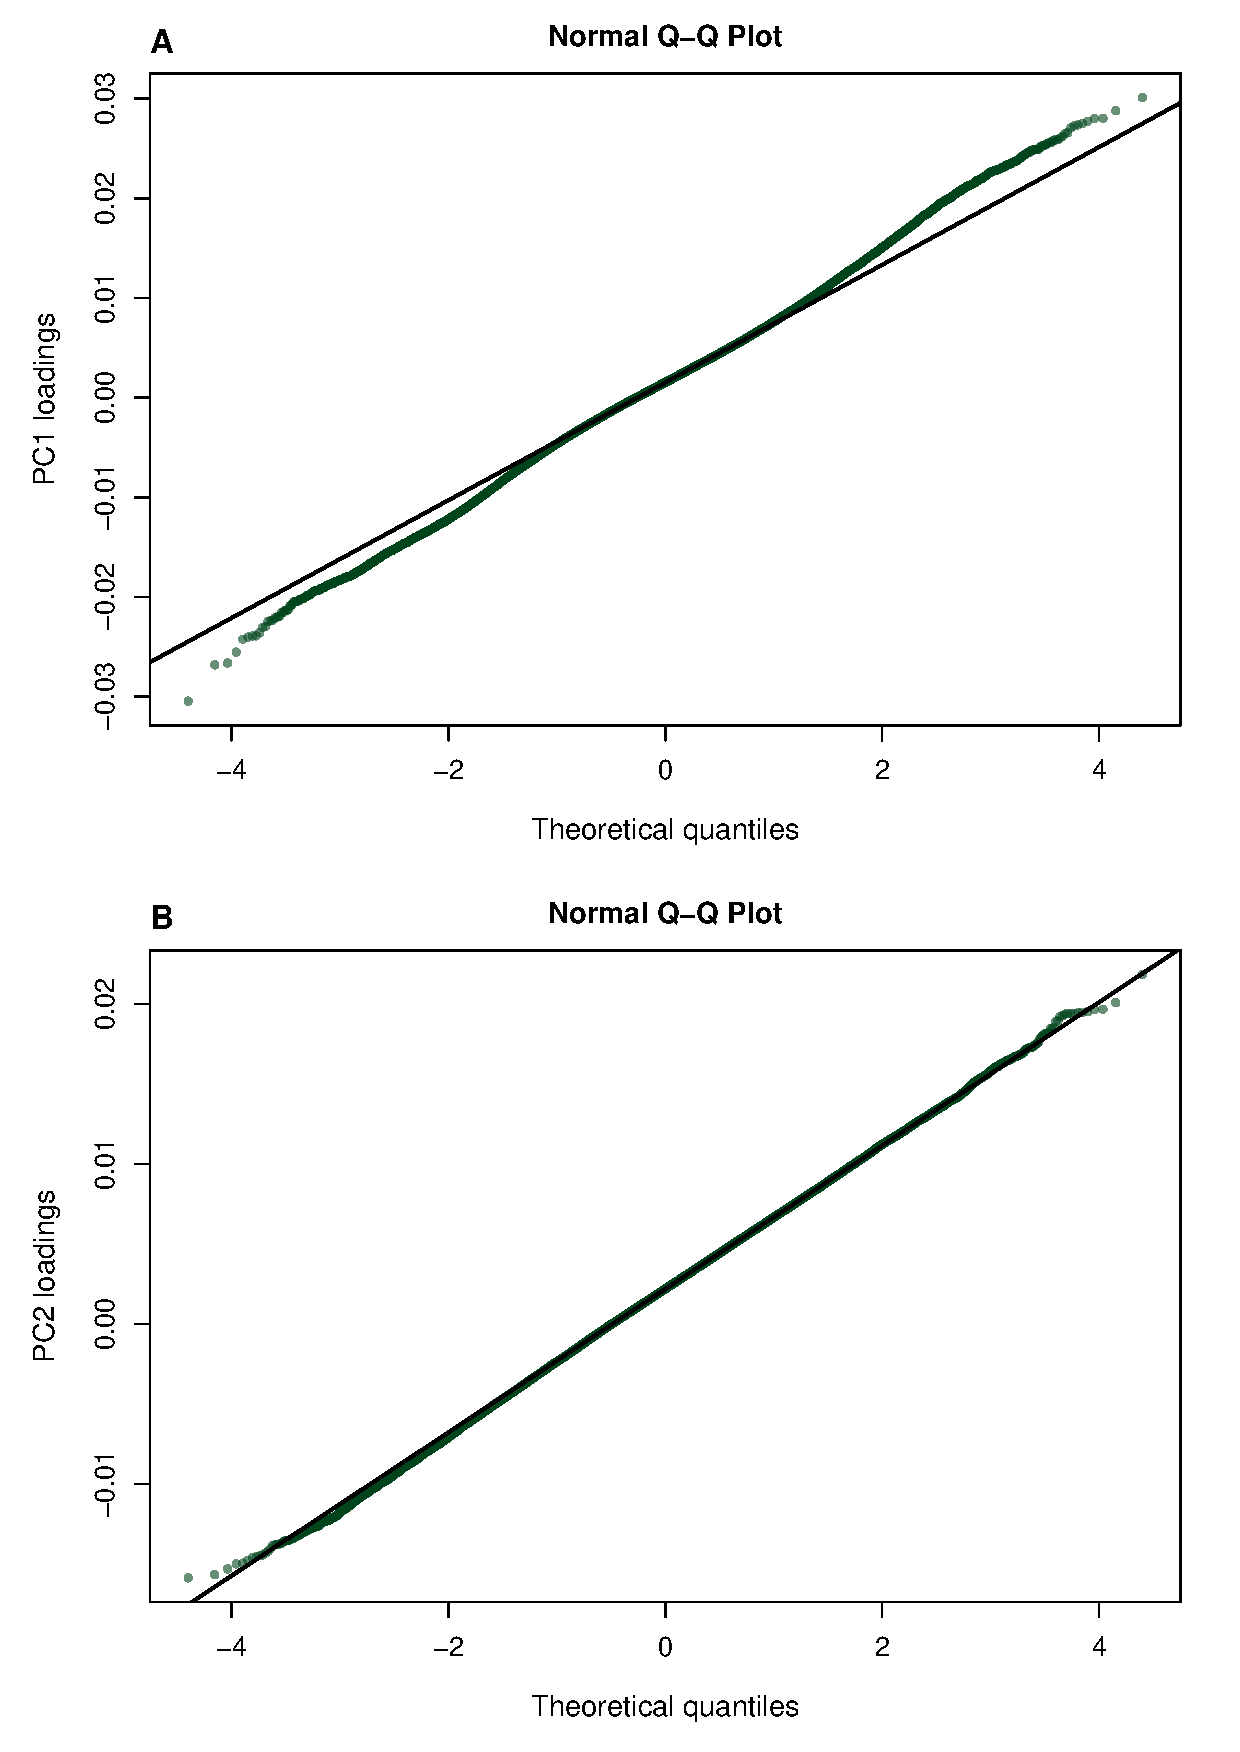
\includegraphics[width=\linewidth]{Figure_S2.pdf}
\captionsetup{justification=raggedright,singlelinecheck=false,width=\linewidth}
\captionof{figure}{Q–Q plots of SNP loadings for PC1 (A) and PC2 (B) against the theoretical normal distribution. PC1 shows mild tail deviations consistent with a weak genome-wide signal along the elevational gradient, whereas PC2 closely follows the null expectation, suggesting predominantly stochastic or technical variation.}
\label{fig:S2}
\end{minipage}
\end{flushleft}
\end{figure}

\begin{figure}[ht]
\begin{flushleft}
\begin{minipage}{0.8\textwidth}
\includegraphics[width=\linewidth]{Figure_S3.pdf}
\captionsetup{justification=raggedright,singlelinecheck=false,width=\linewidth}
\captionof{figure}{Results of Evanno's method for determining the optimal number of genetic clusters (K) for \textit{Isophya rizeensis} along an altitudinal gradient showing $\Delta$K values for different Ks, with peak value indicating the best-supported K.}
\label{fig:S3}
\end{minipage}
\end{flushleft}
\end{figure}

\begin{figure}[ht]
\begin{flushleft}
\begin{minipage}{1\textwidth}
\includegraphics[width=\linewidth]{Figure_S4.pdf}
\captionsetup{justification=raggedright,singlelinecheck=false,width=\linewidth}
\captionof{figure}{Admixture proportions for K=2 to K=5, illustrating genetic ancestries of \textit{Isophya rizeensis} along an altitudinal gradient.}
\label{fig:S4}
\end{minipage}
\end{flushleft}
\end{figure}

\begin{figure}[ht]
\begin{flushleft}
\begin{minipage}{1\textwidth}
\includegraphics[width=\linewidth]{Figure_S5.pdf}
\captionsetup{justification=raggedright,singlelinecheck=false,width=\linewidth}
\captionof{figure}{Genome-wide genetic differentiation of \textit{I. rizeensis} along the altitudinal gradient, measured as pairwise weighted Fst values between collection sites.}
\label{fig:S4}
\end{minipage}
\end{flushleft}
\end{figure}

\begin{figure}[ht]
\begin{flushleft}
\begin{minipage}{1\textwidth}
\includegraphics[width=\linewidth]{Figure_S6.pdf}
\captionsetup{justification=raggedright,singlelinecheck=false,width=\linewidth}
\captionof{figure}{Posterior assignment probabilities of individuals to dark and pale colour morphs inferred from DAPC, plotted along the elevation gradient. Prior groupings are indicated by the color bars up top.}
\label{fig:S4}
\end{minipage}
\end{flushleft}
\end{figure}

\end{document}
